\documentclass[a4paper]{oblivoir}

\title{쟤료공학개론 과제7}
\author{2018-12432, Electrical and Computer Engineering department, ParkJeonghyun}
\date{11/15/2023}

\newcommand{\be}{\begin{equation}}
\newcommand{\ee}{\end{equation}}

\usepackage{fapapersize}
\usepackage{amsmath}
\usepackage{MnSymbol}
\usepackage{wasysym}
\usepackage{graphicx}
\usepackage{caption}
\usepackage{subfig}
\usepackage{hyperref}
\usepackage{cite}
\usepackage{dtk-logos}
\usepackage{physics}
\usepackage{tikz}
\usetikzlibrary{decorations.markings, positioning}
\usepackage{dtk-logos}
\usepackage{fancyvrb}
\usepackage{array} 
\usepackage{chemformula}

\usefapapersize{ 210mm, 297mm, 15mm, 15mm, 15mm, 15mm}
\DeclareGraphicsExtensions{.pdf, .png, .jpg}

\renewcommand{\figurename}{Figure}

\begin{document}

\maketitle
\section{Problem 1}
\begin{figure}[htbp]
	\begin{centering}
	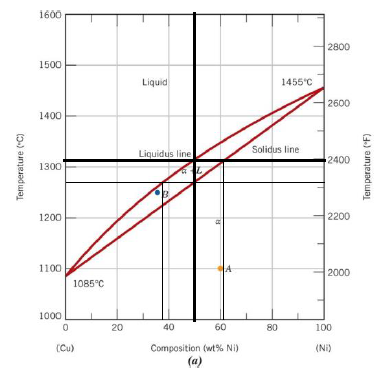
\includegraphics[width = 0.75\linewidth]{pro1.png}% Here is how to import EPS art
	\caption{\label{fig:pro1} \ch{Ni-Co} Phase Diagram}
	\end{centering}
\end{figure}
\subsection{a}
약 $1320^{o}C$에서 발생한다.

\subsection{b}
\ch{Ni} 62\%, \ch{Cu} 38\%이다.

\subsection{c}
약 $1270^{o}C$에서 발생한다.

\subsection{b}
\ch{Ni} 36\%, \ch{Cu} 64\%이다.

\section{Problem 2}
\begin{figure}[htbp]
	\begin{centering}
	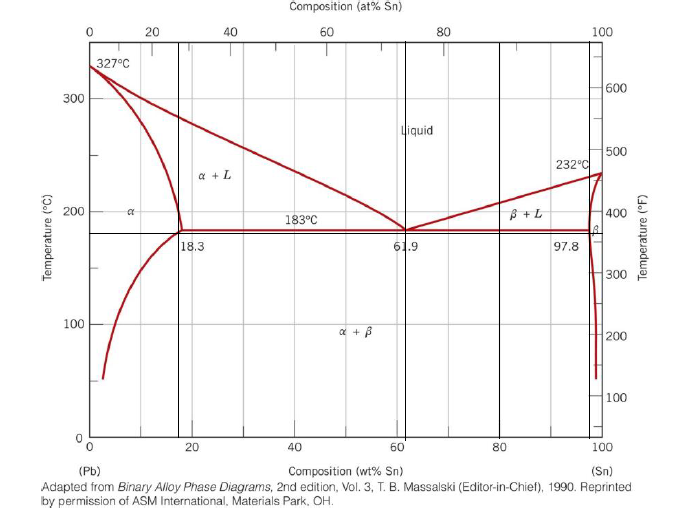
\includegraphics[width = 0.75\linewidth]{pro2.png}% Here is how to import EPS art
	\caption{\label{fig:pro2} \ch{Sn-Pb} Phase Diagram}
	\end{centering}
\end{figure}

\subsection{a}
\begin{align}
	W_{\alpha} &= \frac{97.8-80}{97.8-18.3}\\
	&= 0.224
\end{align}
\begin{align}
	W_{\beta} &= \frac{80-18.3}{97.8-18.3}\\
	&= 0.776
\end{align}

\subsection{b}
\begin{align}
	W_{primary \beta} &= \frac{80-61.9}{97.8-61.9}\\
	&= 0.504
\end{align}
\begin{align}
	W_{eutectic} &= \frac{97.8- 80}{97.8-61.9}\\
	&= 0.496
\end{align}

\subsection{c}
\begin{align}
	W_{eutectic\beta} &= W_{\beta} - W_{primary \beta}\\
	&= 0.776-0.504\\
	&= 0.272
\end{align}

\section{Problem 3}
각 온도별 schematic은 Figs.\ref{fig:pro3_1}, \ref{fig:pro3_2}, \ref{fig:pro3_3}와 같다.
\begin{figure}[htbp]
	\begin{centering}
	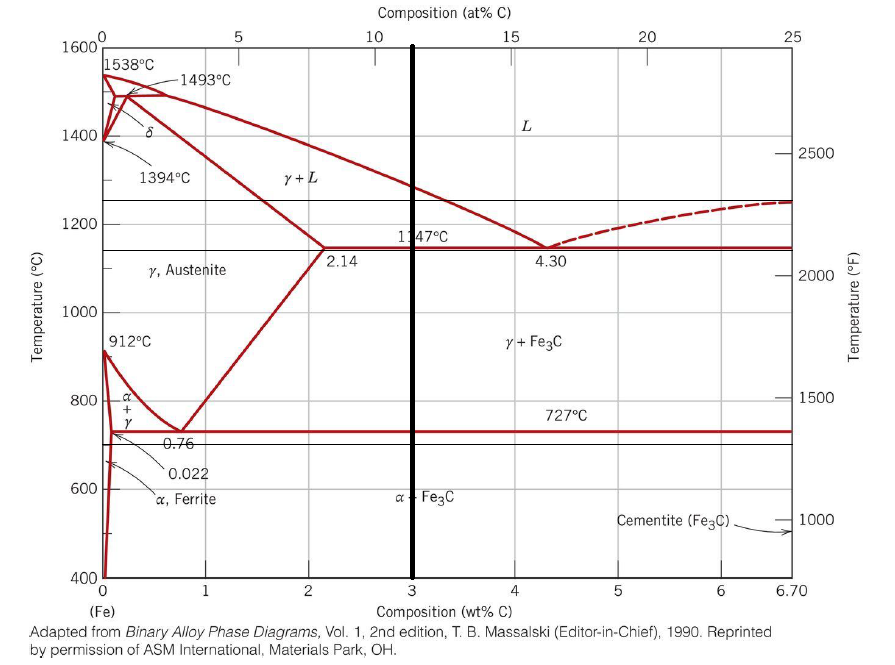
\includegraphics[width = 0.75\linewidth]{pro3.png}% Here is how to import EPS art
	\caption{\label{fig:pro3} \ch{Fe} Phase Diagram}
	\end{centering}
\end{figure}
\begin{figure}[htbp]
	\begin{centering}
	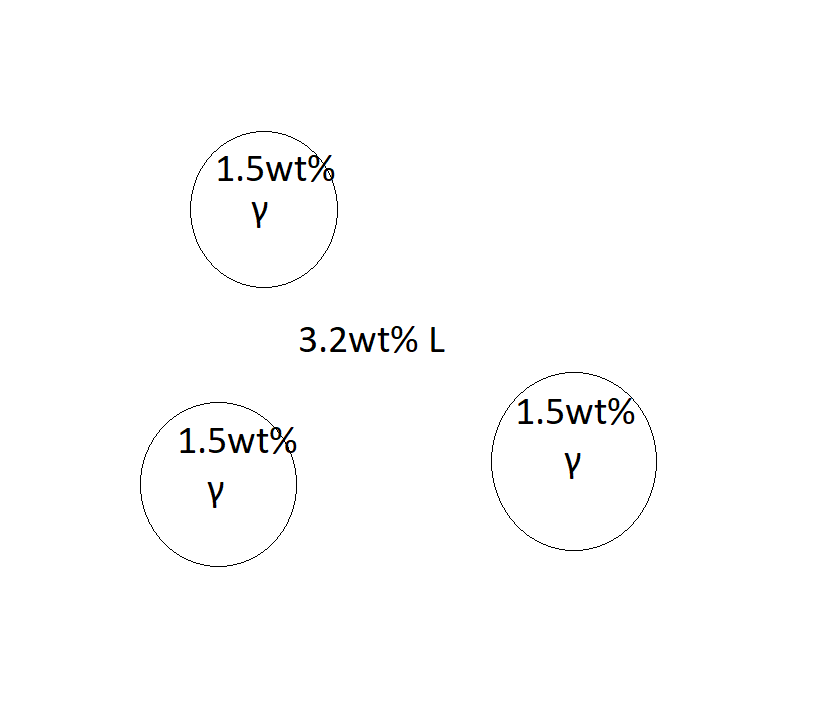
\includegraphics[width = 0.75\linewidth]{pro3_1.png}% Here is how to import EPS art
	\caption{\label{fig:pro3_1} $1250^{o}C$}
	\end{centering}
\end{figure}
\begin{figure}[htbp]
	\begin{centering}
	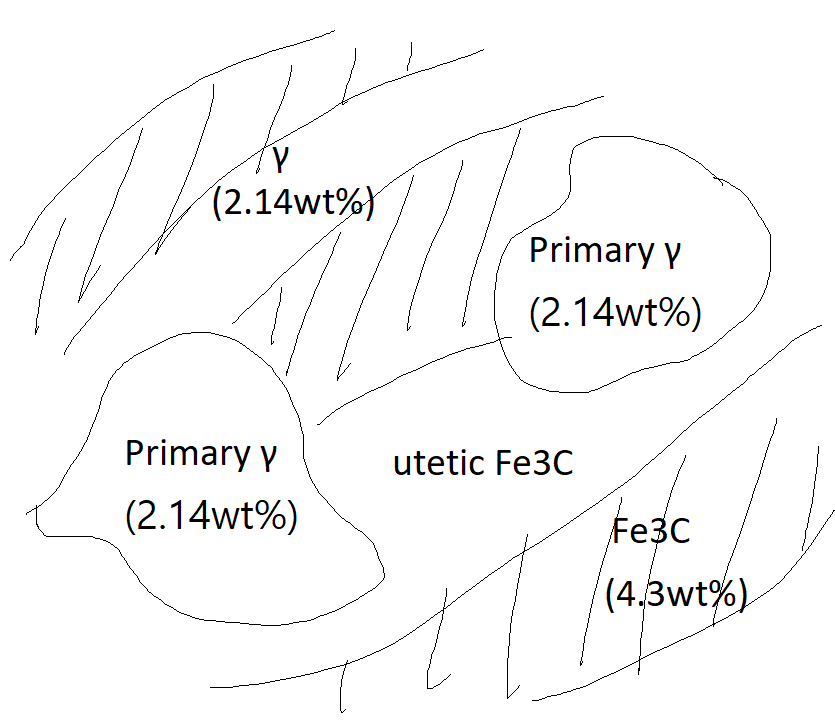
\includegraphics[width = 0.75\linewidth]{pro3_2.png}% Here is how to import EPS art
	\caption{\label{fig:pro3_2} $1145^{o}C$}
	\end{centering}
\end{figure}
\begin{figure}[htbp]
	\begin{centering}
	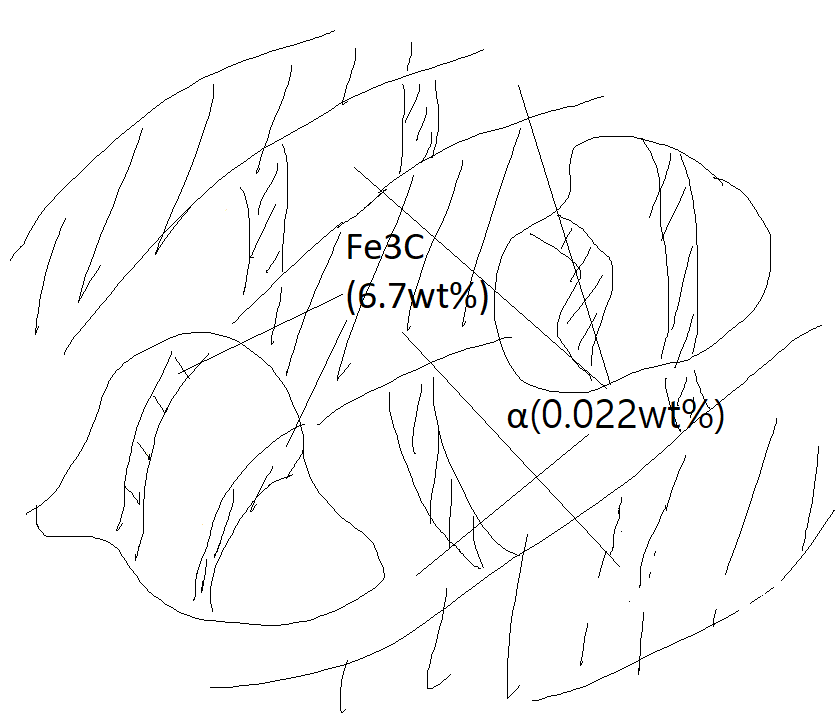
\includegraphics[width = 0.75\linewidth]{pro3_3.png}% Here is how to import EPS art
	\caption{\label{fig:pro3_3} $700^{o}C$}
	\end{centering}
\end{figure}

\end{document}